\begin{figure}
%	\setlength\abovecaptionskip{0.5\baselineskip}
%  	\setlength\abovecaptionskip{0.75\baselineskip}
        \begin{center}
    		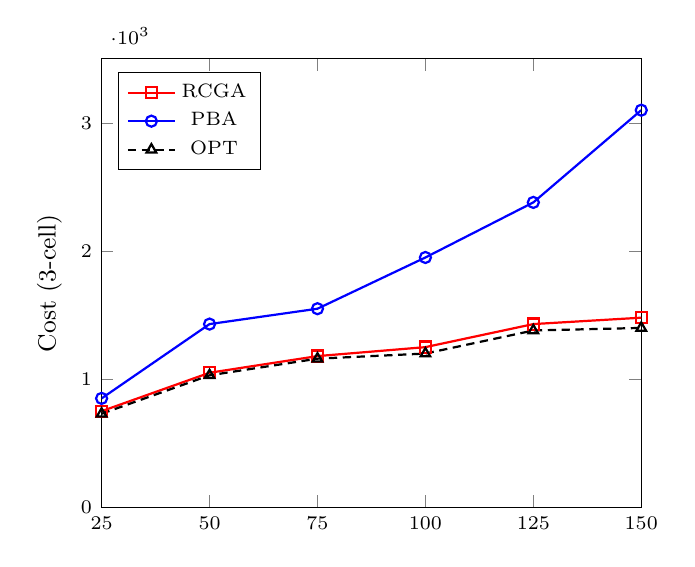
\begin{tikzpicture}
        		\begin{axis}[
        		%	scaled ticks=true, 
        		%	scaled y ticks={real:1e3},
        			scaled y ticks=base 10:-3,
        		    %title={},
        		%    xlabel={The number of contents $I$},
        		    ylabel={Cost (3-cell)},
        		    xmin=25, xmax=150,
        		    ymin=0, ymax=3500,
        		    xtick={25, 50, 75, 100, 125, 150},
        		%	xticklabels=\empty,
        %		    ytick={0, 1000, 2000, 3000},
        		%	point meta=y *10^3, % the displayed number
        		    legend pos=north west,
        		    %ymajorgrids=true,    
        		    %xmajorgrids=true,
        		    grid style=densely dashed,
        		    tick label style={font=\scriptsize},
        		    label style={font=\small},
        		    legend style={font=\scriptsize},
        		]
        		
            		\addplot[ color=red, mark=square, line width=0.8pt]     
            		coordinates { (25, 750) (50, 1050) (75, 1180) (100, 1250) (125, 1430) (150, 1480) };
            		%
            		\addplot[ color=blue, mark=o, mark options={solid}, line width=0.8pt]     
            		coordinates { (25, 850) (50, 1430) (75, 1550) (100, 1950) (125, 2380) (150, 3100) };
            		
            		\addplot[ color=black, mark=triangle, densely dashed, mark options={solid}, line width=0.8pt]
            		coordinates { (25, 730) (50, 1030) (75, 1160) (100, 1200) (125, 1380) (150, 1400) };
            		
            		\legend{RCGA, PBA, OPT}
        		
        		\end{axis}
    		\end{tikzpicture}
    		
        \end{center}
    \caption{Caption.}\label{fig:result2}
\end{figure}
